\documentclass[11pt,a4paper]{article}
\usepackage[T1]{fontenc}
\usepackage[margin=2.3cm]{geometry}
\usepackage{amsmath,amssymb}
\usepackage{graphicx}
\usepackage[dvipsnames]{xcolor}
\usepackage{enumitem}
\usepackage[colorlinks=true,linkcolor=blue,urlcolor=blue]{hyperref}
\setlength{\parskip}{0.6em}
\setlength{\parindent}{0pt}
\begin{document}

\begin{center}{\LARGE\bfseries openexperiment}\\[0.4em]{\large Design a fair experiment and calibrate a sensor, in three sessions.}\\[0.2em]\small PAN IIT OSS explainer \textbullet{} higher secondary to advanced undergraduate (levels 4-6)\end{center}

\section*{Why this exists}
Every measurement is a number plus an uncertainty, and every comparison is only as fair as the way it was run. This explainer shows the mathematics behind fair tests, sensor calibration and experimental design, using a simulated sensor so every claim can be checked against the truth.

\section*{The end goal}
Design a fair experiment and calibrate a sensor. The end goal is to design a fair experiment and calibrate a sensor: to plan the runs so that drift and confounding cannot fool you, and to turn raw readings into values with honest uncertainties. The same habits apply to laboratory work, engineering tests and data science.

\section*{How the three sessions build up}
\begin{enumerate}[nosep]
\item \textbf{Session 1: A fair test: one change, repeated, and accurate versus precise} (Level 1, conceptual interactive model, 60 min).
\item \textbf{Session 2: Calibrating a sensor: a line, its uncertainty, and how many readings} (Level 2, mathematical engineering model, 80 min).
\item \textbf{Session 3: Designing the experiment: order, replicates, factors and drift} (Level 3, simulation and validation, 90 min).
\end{enumerate}

\section{Session 1: A fair test: one change, repeated, and accurate versus precise}

\subsection*{A. Real-world problem}
You want to know whether a lid keeps a cup of hot water warmer. You put the lid on a big cup and leave a small cup bare. The covered cup cools less, so the lid works, right? Not necessarily: the big cup would have cooled less anyway. And if you ran the test only once, a lucky or unlucky run could fool you. This session builds a made-up world where the true answer is known, so you can see exactly how unfair and one-off tests go wrong. This is general education about experiments.

\subsection*{B. Concept and theory}
A fair test changes one thing (the lid) and keeps everything else the same (same cup, same water, same time, same thermometer, same way of reading it). Every measurement also has scatter, so we repeat the test and use the mean of the n repeats: the mean's scatter is sd / sqrt(n). The effect of the lid is the mean with the lid minus the mean without. Two words describe a measuring instrument. Accurate means that its readings average close to the truth: its bias (average error) is small. Precise means that repeated readings agree with each other: their scatter (standard deviation) is small. Bias and scatter are independent: all four combinations exist.

\begin{itemize}[nosep]
\item lid effect: true change in cooling drop caused by the lid (-1.0) (degrees C)
\item cup effect: true change caused by a big cup (-3.0) (degrees C)
\item sd: scatter of one measurement (1.5 for the cooling test) (degrees C)
\item n: repeats per setting (no unit)
\item bias: average reading minus the truth (degrees C)
\end{itemize}

\begin{equation*}
\text{effect}=\bar y_{\text{lid}}-\bar y_{\text{bare}},\qquad \mathrm{sd}(\bar y)=\frac{\sigma}{\sqrt n}
\end{equation*}

\begin{equation*}
\mathrm{sd}(\bar y_1-\bar y_2)=\sigma\sqrt{\frac{2}{n}}
\end{equation*}

\begin{equation*}
P(\text{wrong sign})=P\!\left(Z>\frac{|\text{effect}|}{\sigma\sqrt{2/n}}\right)
\end{equation*}

\begin{equation*}
\text{typical error}=\sqrt{\text{bias}^2+\left(\frac{\sigma}{\sqrt n}\right)^2}
\end{equation*}

\begin{center}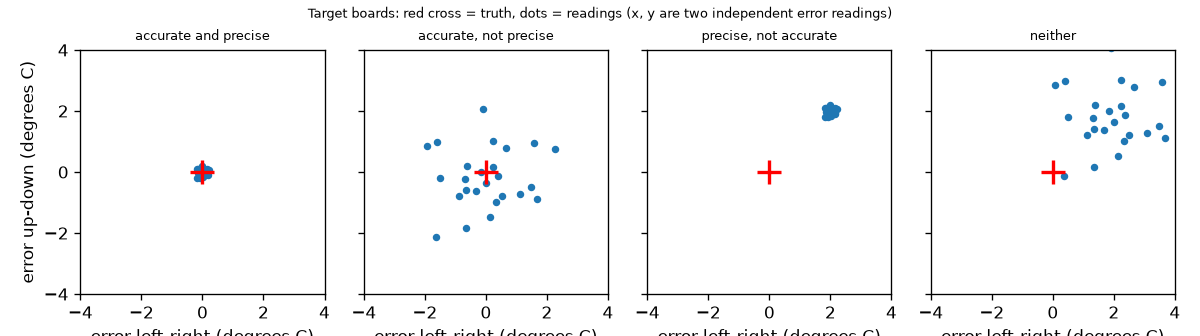
\includegraphics[width=0.85\linewidth]{figures/s01_accurate_precise.png}\\\small Four thermometers as target boards: bias moves the cluster, scatter widens it.\end{center}

\subsection*{E. Worked example}
In the made-up cooling test the lid effect is -1.0 degrees C and the scatter is 1.5 degrees C per run. (a) What does the unfair test (lid on the big cup against a bare small cup) report? (b) With one run per setting in a fair test, what is the chance of the wrong sign?
\begin{enumerate}[nosep]
\item Unfair test, no scatter: (20 - 1 - 3) - 20 = -4 degrees C. It reports -4, but the lid is only -1; the extra -3 is the cup size.
\item Fair test, no scatter: (20 - 1) - 20 = -1 degrees C: the true lid effect.
\item With n = 1 the difference of two runs has scatter 1.5 * sqrt(2) = 2.12 degrees C.
\item A wrong sign needs the difference to exceed 0, that is a shift of 1 / 2.12 = 0.471 standard deviations: the normal tail beyond 0.471 is 0.319.
\end{enumerate}
\textbf{Answer.} The unfair test gives -4 (wrong by the cup effect, -3). A one-run fair test says the lid makes things worse in 0.319 of cases, about one time in three. With 9 runs per setting this falls to 0.079.

\subsection*{F. Questions}
\begin{enumerate}[nosep]
\item \textbf{Conceptual.} A friend says: 'My plant food works: the plants I fed in the sunny window grew taller than the unfed ones on the shelf.' What is wrong with this test, and how would you fix it?
\item \textbf{Numerical.} In the cooling test (lid effect -1.0 degrees C, scatter 1.5 degrees C per run) you use n = 9 runs per setting. What is the scatter of the difference of the two means, and the chance of getting the wrong sign?
\item \textbf{Graph and simulation interpretation.} In the app graph view, bias is 2.0, sd is 1.0 and you move n from 1 to 100. Describe the black curve and what limits it.
\item \textbf{Design and optimisation challenge.} Design: you have a thermometer with bias 2.0 degrees C and sd 0.1 degrees C, and another with bias 0 and sd 1.0 degrees C. You can afford at most 25 readings in total. Which do you choose to measure a temperature to within 0.5 degrees C, and what do you do with the first one?
\end{enumerate}

\section{Session 2: Calibrating a sensor: a line, its uncertainty, and how many readings}

\subsection*{A. Real-world problem}
A cheap temperature sensor reports 1.02 times the true temperature minus 0.8 degrees, plus noise. You do not know that; you only have its readings and a trusted reference thermometer. How do you turn a reading of 30.4 into a temperature, and how uncertain is the answer? How many readings must you average to know a temperature to within 0.1 degrees? This is general education about measurement, not a procedure for a safety-critical instrument.

\subsection*{B. Concept and theory}
Calibration: measure n known reference values x with the sensor to get readings y, and fit the line y = m x + c by least squares. With Sxx = sum (x - xbar)\textasciicircum{}2, Sxy = sum (x - xbar)(y - ybar): m = Sxy / Sxx and c = ybar - m xbar. The residual scatter is s = sqrt(sum residual\textasciicircum{}2 / (n - 2)); the standard errors are SE(m) = s / sqrt(Sxx) and SE(c) = s sqrt(1/n + xbar\textasciicircum{}2 / Sxx). Inverse prediction: a new reading y0 (the mean of k readings) is turned into x0 = (y0 - c) / m with uncertainty u = (s / \textbar{}m\textbar{}) sqrt(1/k + 1/n + (x0 - xbar)\textasciicircum{}2 / Sxx), smallest in the middle of the calibrated range. Repeatability is the scatter of repeats under the same conditions; reproducibility includes changes of day or set-up, so reproducibility sd = sqrt(repeatability\textasciicircum{}2 + between-day sd\textasciicircum{}2). An N-bit ADC over a range lo to hi has LSB = (hi - lo) / 2\textasciicircum{}N and a rounding error with sd LSB / sqrt(12). Averaging N readings leaves bias unchanged and shrinks the random error to sd / sqrt(N); to reach a 95 percent half-width h we need N \textgreater{}= (1.96 sd / h)\textasciicircum{}2.

\begin{itemize}[nosep]
\item x: reference (true) temperature (degrees C)
\item y: sensor reading (degrees C)
\item m, c: calibration slope (no unit) and intercept (degrees C per degree C, degrees C)
\item s: residual scatter about the line (degrees C)
\item Sxx: sum of squared distances of x from its mean (degrees C squared)
\item u(x0): standard uncertainty of the inverted value (degrees C)
\item LSB: ADC step (degrees C)
\item N, k: number of readings averaged (no unit)
\end{itemize}

\begin{equation*}
m=\frac{S_{xy}}{S_{xx}},\qquad c=\bar y-m\bar x,\qquad s=\sqrt{\frac{\sum (y_i-mx_i-c)^2}{n-2}}
\end{equation*}

\begin{equation*}
\mathrm{SE}(m)=\frac{s}{\sqrt{S_{xx}}},\qquad \mathrm{SE}(c)=s\sqrt{\frac1n+\frac{\bar x^2}{S_{xx}}}
\end{equation*}

\begin{equation*}
x_0=\frac{y_0-c}{m},\qquad u(x_0)=\frac{s}{|m|}\sqrt{\frac1k+\frac1n+\frac{(x_0-\bar x)^2}{S_{xx}}}
\end{equation*}

\begin{equation*}
\mathrm{LSB}=\frac{\text{hi}-\text{lo}}{2^N},\qquad \sigma_q=\frac{\mathrm{LSB}}{\sqrt{12}}
\end{equation*}

\begin{equation*}
\sigma_{\text{repro}}=\sqrt{\sigma_{\text{repeat}}^2+\sigma_{\text{day}}^2},\qquad N\ge\left(\frac{1.96\,\sigma}{h}\right)^2
\end{equation*}

\begin{center}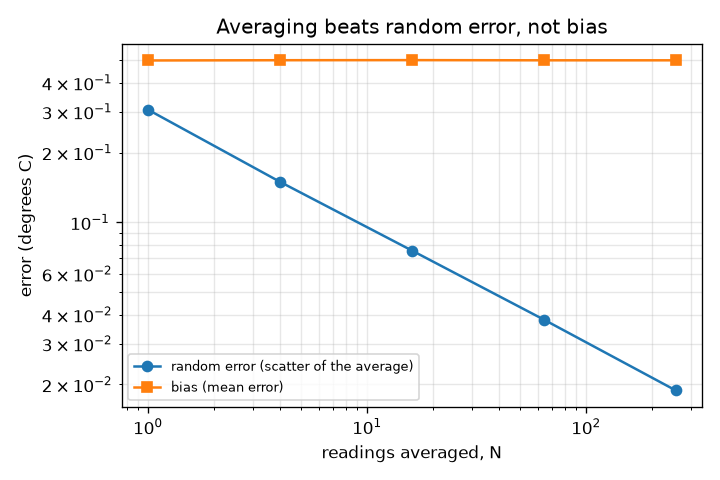
\includegraphics[width=0.85\linewidth]{figures/s02_average_vs_bias.png}\\\small Averaging N readings shrinks the random error as 1 / sqrt(N); the bias of 0.5 degrees C stays.\end{center}

\subsection*{E. Worked example}
A calibration with 11 points (0 to 100 degrees C) gave slope 1.02, intercept -0.80 degrees C and s = 0.30 degrees C. The sensor now reads 30.4 degrees C. (a) What is the true temperature and its standard uncertainty? (b) How much better is the average of 4 readings? (c) How many readings are needed to know a mean to +-0.1 degrees C at 95 percent when the scatter is 0.30?
\begin{enumerate}[nosep]
\item x0 = (30.4 - (-0.80)) / 1.02 = 31.2 / 1.02 = 30.59 degrees C.
\item Sxx = 11000, xbar = 50, so (x0 - xbar)\textasciicircum{}2 / Sxx = (30.59 - 50)\textasciicircum{}2 / 11000 = 0.0343.
\item k = 1: u = (0.30 / 1.02) sqrt(1 + 1/11 + 0.0343) = 0.2941 * 1.061 = 0.312 degrees C.
\item k = 4: u = 0.2941 * sqrt(0.25 + 0.0909 + 0.0343) = 0.2941 * 0.6126 = 0.180 degrees C: better, but not 4 times better, because the calibration line itself stays uncertain.
\item Readings needed: N \textgreater{}= (1.96 * 0.30 / 0.1)\textasciicircum{}2 = 5.88\textasciicircum{}2 = 34.57, rounded up to 35.
\end{enumerate}
\textbf{Answer.} True temperature 30.59 degrees C with u = 0.31 degrees C (one reading) or 0.18 degrees C (mean of 4); 35 readings are needed for +-0.1 degrees C at 95 percent (34 readings reach only 0.948, 35 reach 0.951).

\subsection*{F. Questions}
\begin{enumerate}[nosep]
\item \textbf{Conceptual.} Why is the uncertainty of the inverted temperature smallest in the middle of the calibrated range and larger near the ends? Why can you not reduce it to zero by averaging the new readings?
\item \textbf{Numerical.} A sensor has scatter sd = 1.0 degrees C. How many readings must be averaged to know the mean to +-0.2 degrees C at 95 percent, and how many for +-0.1?
\item \textbf{Graph and simulation interpretation.} In the average-versus-bias figure the scatter line falls with slope -1/2 on log axes while the bias line is flat. What does each tell you, and which could you reduce by taking more readings?
\item \textbf{Design and optimisation challenge.} Design: a 10-bit ADC over 0 to 100 degrees C is available. Its sensor noise sd is 0.30 degrees C. Is the quantisation noise a problem compared with the sensor noise? Would an 8-bit ADC be acceptable? Justify with numbers.
\end{enumerate}

\section{Session 3: Designing the experiment: order, replicates, factors and drift}

\subsection*{A. Real-world problem}
You must compare two treatments with a sensor that slowly drifts upward while you work. If you run all of treatment A first and all of B afterwards, B looks better even when it does nothing. How should the 20 runs be ordered? How many runs do you need to see a small effect? And what if two factors only help when changed together? This session tests each design on a simulated world where the true answer is known. It is general education, not a template for a regulated or safety-critical test.

\subsection*{B. Concept and theory}
Randomisation, balance and blocking protect against nuisance factors such as drift. With a straight-line drift of r per run, the effect estimate (mean B minus mean A) is biased by r times (mean run number of B minus mean run number of A): 10 r when all A runs come first, 0 for an ABBA pattern. Under complete random order the bias is zero on average, but the drift adds scatter: for 20 runs with 10 per treatment the added variance is 7 r\textasciicircum{}2. Pairing runs and randomising within each pair (randomised blocks) keeps almost none of it. Replication: for a two-sided z-test at 5 percent significance with power 80 percent, n = 2 (z\_a + z\_b)\textasciicircum{}2 sigma\textasciicircum{}2 / d\textasciicircum{}2 runs per group detect a difference d (z\_a = 1.96, z\_b = 0.8416). Factorial design: a 2x2 design runs all four corners of two factors at coded levels -1 and +1; main effect A = mean(A high) - mean(A low), interaction AB = half the difference of A's effect at B high and B low. One-factor-at-a-time changes one factor from a start and keeps the better; with an interaction it can stop at a worse setting. Calibration drift: if the offset error after calibration has standard uncertainty u and then drifts at rate r, keep 1.96 u + r t within the tolerance. A line fitted in one range must not be used outside it if the sensor curves.

\begin{itemize}[nosep]
\item r: drift per run (0.05) or per day (0.02) (degrees C per run or per day)
\item d: true difference between group means (same unit as the response)
\item sigma: scatter of one run (same unit as the response)
\item n: runs per group (no unit)
\item z\_a, z\_b: normal points for significance (1.96) and power (0.8416) (no unit)
\item A, B: coded factor levels (-1 or +1)
\item u: uncertainty of the offset just after calibration (degrees C)
\item tol: allowed error (degrees C)
\end{itemize}

\begin{equation*}
\text{bias}=r\,(\bar t_B-\bar t_A),\qquad \text{(all A first: } 10r\text{; ABBA: } 0)
\end{equation*}

\begin{equation*}
n=\frac{2\,(z_{\alpha}+z_{\beta})^2\sigma^2}{d^2},\qquad \text{power}=\Phi\!\left(\frac{d}{\sigma\sqrt{2/n}}-z_\alpha\right)
\end{equation*}

\begin{equation*}
E_A=\tfrac12\,(y_{+-}+y_{++}-y_{--}-y_{-+}),\qquad E_{AB}=\tfrac12\,(y_{--}+y_{++}-y_{+-}-y_{-+})
\end{equation*}

\begin{equation*}
t_{\max}=\left\lfloor\frac{\text{tol}-1.96\,u}{r}\right\rfloor,\qquad y=b_0+b_1T+b_2\,\Delta V+b_3\,T\,\Delta V
\end{equation*}

\begin{center}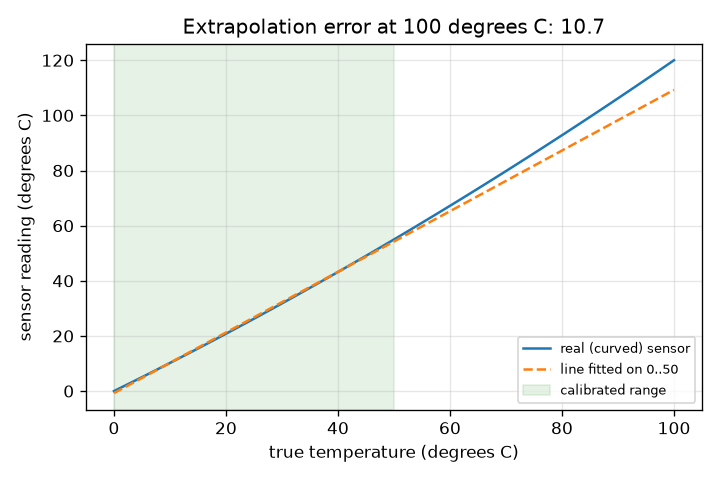
\includegraphics[width=0.85\linewidth]{figures/s03_extrapolation.png}\\\small A line fitted on 0 to 50 degrees C fails outside the calibrated range of a curved sensor.\end{center}

\subsection*{E. Worked example}
Treatment B truly raises the response by 0.30 degrees C. The sensor drifts by 0.05 degrees C per run and one run has scatter 0.50. Twenty runs: 10 of A and 10 of B. (a) What bias does the all-A-then-all-B order have? (b) How many runs per group would detect a difference d = 0.5 with sigma = 1.0 at 5 percent significance and 80 percent power? (c) In the 2x2 system response = 50 + A + B + 6AB, what are the effects, and where does one-factor-at-a-time stop?
\begin{enumerate}[nosep]
\item (a) Mean run number of A is 4.5, of B is 14.5: bias = 0.05 * (14.5 - 4.5) = 0.50 degrees C, bigger than the true effect 0.30.
\item Noise alone gives scatter 0.50 * sqrt(2 / 10) = 0.2236; complete randomisation adds drift scatter 0.05 * sqrt(7) = 0.132, total sqrt(0.2236\textasciicircum{}2 + 0.132\textasciicircum{}2) = 0.260.
\item (b) n = 2 * (1.96 + 0.8416)\textasciicircum{}2 * 1.0\textasciicircum{}2 / 0.5\textasciicircum{}2 = 2 * 7.849 / 0.25 = 62.79, rounded up to 63 runs per group.
\item (c) The four runs (-,-), (+,-), (-,+), (+,+) give 54, 44, 44, 58. A = ((44 + 58) - (54 + 44)) / 2 = 2, B = 2, AB = ((54 + 58) - (44 + 44)) / 2 = 12.
\item One-factor-at-a-time starts at (-,-) = 54: raising A gives 44 (worse), raising B gives 44 (worse), so it stops at 54; the best is (+,+) = 58.
\end{enumerate}
\textbf{Answer.} (a) A bias of 0.50 degrees C. (b) 63 runs per group (power 0.801; 62 give 0.795). (c) Effects 2, 2 and 12; one-factor-at-a-time stops at 54 and misses the best setting 58.

\subsection*{F. Questions}
\begin{enumerate}[nosep]
\item \textbf{Conceptual.} Why does randomising the run order protect an experiment against drift you did not know about, while ABBA only protects against straight-line drift? What does randomisation cost?
\item \textbf{Numerical.} How many runs per group are needed to detect a difference d = 0.25 with sigma = 1.0 at 5 percent significance and 80 percent power? Compare with d = 0.5 (63 runs).
\item \textbf{Graph and simulation interpretation.} In the interaction figure the two lines are not parallel. What does this say about the effect of factor A, and why does one-factor-at-a-time fail here?
\item \textbf{Design and optimisation challenge.} Design: after calibration the offset uncertainty is 0.10 degrees C, the drift is 0.02 degrees C per day and the allowed error is 0.50 degrees C. How often must you recalibrate? What happens after 20 days? What if the tolerance were 0.10?
\end{enumerate}

\section{Real-world mini-project}
\textbf{Calibrate a sensor across temperature and supply voltage.} A made-up sensor reads 0.98 T + 0.5 + (V - 5)(0.8 + 0.004 T) plus a drift of 0.01 degrees C per run and noise with sd 0.30 degrees C, where T is the true temperature (degrees C) and V the supply voltage (volts). Use \texttt{run\_experiment}, \texttt{two\_factor\_effects}, \texttt{fit\_two\_factor} and \texttt{estimate\_T} from Session 3. Run the 2x2 design (T = 20 and 80 degrees C, V = 4.5 and 5.5 V, 5 runs per corner in randomised blocks), report the effects, fit the calibration, and compare the temperature error of one new reading at 50 degrees C and 5.4 V when the voltage is in the model and when it is ignored.

\section{The path ahead}
\begin{enumerate}[nosep]
\item \textbf{Session 4: Calibrate a curved sensor.} A calibration routine that fits a straight line and a quadratic, picks one by looking at the residuals, and inverts it.
\item \textbf{Session 5: Uncertainty budget for one reading.} A function that returns the combined standard uncertainty of a temperature reading from its sources and the average of k readings.
\item \textbf{Session 6: Fewer runs: a fractional factorial.} A 2\textasciicircum{}(3-1) design of 4 runs per replicate that estimates three main effects of a made-up sensor.
\item \textbf{Session 7: A drift-aware recalibration schedule.} A simulation of random-walk drift that reports the longest interval keeping the chance of exceeding the tolerance below 1 percent.
\item \textbf{Session 8: Calibrate real hardware.} The same pipeline (fit, standard errors, inverse prediction, bootstrap) applied to real readings taken at three or more reference temperatures.
\end{enumerate}

\section{Answers and hints}

\subsection*{Session 1}
\begin{enumerate}[nosep]
\item \textbf{Conceptual.} Hint: List everything that differs between the two groups, not just the food. Solution: Two things changed: the food and the position (sunlight). The extra growth may come from the sun. A fair test puts all plants in the same place, changes only the food, uses several plants per group (repeats) and measures them the same way. Like the lid on the big cup, the effect of food cannot be separated from sunlight when both change together.
\item \textbf{Numerical.} Hint: Scatter of the difference = 1.5 * sqrt(2 / n). Then z = 1 / that, and use the normal tail. Solution: Scatter = 1.5 * sqrt(2 / 9) = 0.707 degrees C. z = 1 / 0.707 = 1.414, and the normal tail beyond 1.414 is 0.079. Units: degrees C. Sanity check: it is smaller than the 0.319 for one run, as it should be, because more repeats shrink the scatter.
\item \textbf{Graph and simulation interpretation.} Hint: Compare the blue curve (random part) and the red line (bias). Solution: The black curve (typical total error) starts at sqrt(2\textasciicircum{}2 + 1\textasciicircum{}2) = 2.24 at n = 1 and falls, but it flattens at 2.0 (the red line) however large n gets, because averaging shrinks only the random part sd / sqrt(n). To go lower you must remove the bias (calibrate), not take more readings.
\item \textbf{Design and optimisation challenge.} Hint: Compute the typical error sqrt(bias\textasciicircum{}2 + sd\textasciicircum{}2/n) for each. Solution: The second one: with 25 readings its typical error is 1.0 / sqrt(25) = 0.2 degrees C (below 0.5). The first one stays at about 2.0 whatever n is. The first could be fixed by calibrating it against a reference (subtracting its bias), after which its scatter 0.1 degrees C makes it the better instrument. The trade-off is the cost and time of the reference measurement. Assumption: the bias is constant.
\end{enumerate}

\subsection*{Session 2}
\begin{enumerate}[nosep]
\item \textbf{Conceptual.} Hint: Look at the term (x0 - xbar)\textasciicircum{}2 / Sxx and at the 1/n term in the formula. Solution: The fitted line is pinned best near the centre of the data (the mean point xbar, ybar); its tilt error acts like a lever, so errors grow with the distance (x0 - xbar). Averaging k new readings removes only the 1/k term; the calibration terms 1/n and (x0 - xbar)\textasciicircum{}2 / Sxx stay, since they come from the one calibration you made. To lower them, add calibration points.
\item \textbf{Numerical.} Hint: N \textgreater{}= (1.96 sd / h)\textasciicircum{}2 and round up. Solution: For h = 0.2: (1.96 / 0.2)\textasciicircum{}2 = 96.04, so N = 97. For h = 0.1: (1.96 / 0.1)\textasciicircum{}2 = 384.2, so N = 385. Halving the target needs 4 times the readings. Units: sd and h in degrees C, N has no unit. This assumes the bias is zero or already removed.
\item \textbf{Graph and simulation interpretation.} Hint: The scatter follows sd / sqrt(N). Solution: A slope of -1/2 on log-log axes means error proportional to N\textasciicircum{}(-1/2): random error, reduced by averaging (0.30 for N = 1, 0.075 for N = 16 and 0.019 for N = 256). The flat line at 0.5 degrees C is the bias: averaging never reduces it. Only calibration (finding and subtracting it) can.
\item \textbf{Design and optimisation challenge.} Hint: Compute LSB / sqrt(12) for 10 and 8 bits and compare with 0.30. Combine independent errors as the square root of the sum of squares. Solution: 10 bits: LSB = 100 / 1024 = 0.0977 degrees C, quantisation sd = 0.0282, tiny against 0.30 (total sqrt(0.30\textasciicircum{}2 + 0.0282\textasciicircum{}2) = 0.301). 8 bits: LSB = 0.3906, sd = 0.1128 (total sqrt(0.09 + 0.0127) = 0.320, about 7 percent worse). So 8 bits is acceptable if a 7 percent increase in scatter is tolerable and the saving in cost matters; 10 bits is practically free of quantisation error. The sensor noise also helps: noise about one LSB wide lets averaging remove the rounding error.
\end{enumerate}

\subsection*{Session 3}
\begin{enumerate}[nosep]
\item \textbf{Conceptual.} Hint: Think about what each design assumes about the drift, and look at the scatter figure. Solution: Random order breaks the link between treatment and time whatever the drift looks like, so the bias is zero on average for any drift shape. ABBA cancels exactly a drift that is a straight line, but a curved drift is not cancelled exactly. The cost of full randomisation is extra scatter (0.26 against 0.22 degrees C here) because the drift is no longer cancelled in each run. Randomised blocks (random order within each pair) give both: protection and low scatter.
\item \textbf{Numerical.} Hint: n = 2 (1.96 + 0.8416)\textasciicircum{}2 sigma\textasciicircum{}2 / d\textasciicircum{}2. Solution: n = 2 * 7.849 * 1.0 / 0.0625 = 251.2, rounded up to 252. Halving the difference to detect multiplies n by 4 (63 to 252). Units: sigma and d in the same unit, n has no unit. Sanity check: 4 times 62.79 is 251.2.
\item \textbf{Graph and simulation interpretation.} Hint: Read the effect of A (the change along the line) at B = -1 and at B = +1. Solution: At B = -1 raising A lowers the response (54 to 44); at B = +1 it raises it (44 to 58). The effect of A depends on B: that is an interaction (AB = 12). One-factor-at-a-time varies A only at B = -1, sees a decrease and concludes the wrong thing; it never visits (+,+), the best corner.
\item \textbf{Design and optimisation challenge.} Hint: Solve 1.96 * 0.10 + 0.02 t \textless{}= 0.50 for t. The chance of being above +0.50 after t days is the normal tail beyond (0.50 - 0.02 t) / 0.10. Solution: t \textless{}= (0.50 - 0.196) / 0.02 = 15.2, so recalibrate every 15 days: the chance of being above +0.50 is then 0.0228. After 20 days that chance is 0.159. With a tolerance of 0.10 even a fresh calibration (1.96 * 0.10 = 0.196) exceeds it, so no interval works: the calibration uncertainty itself must be reduced (better reference, more points). Trade-off: a shorter interval costs more time and reference use.
\end{enumerate}

\section{How to join}
Read \texttt{CONTRIBUTING.md} in the repository, then pick an issue labelled \texttt{good first issue}. Repository: \url{https://github.com/KrunalPanchal1995/openexperiment}

\end{document}
